\begin{sansmath}
\begin{figure*}[h!]
	\centering
	\hspace*{\fill}
	\begin{subfigure}{.527\textwidth}
		\centering
		\vspace{-1em}
		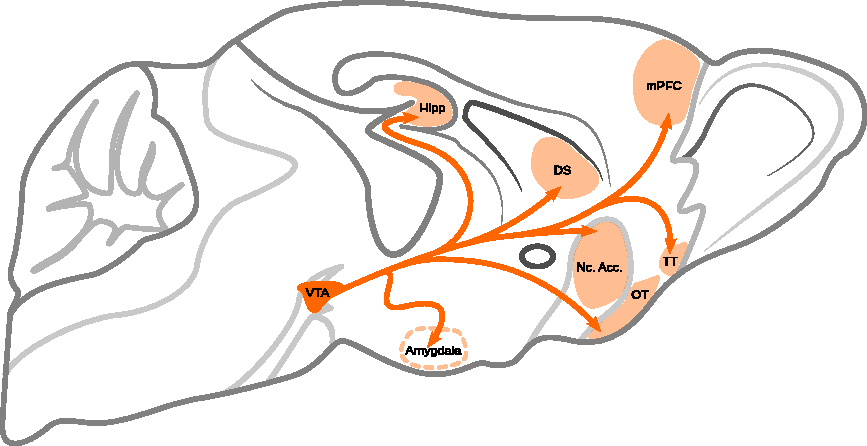
\includegraphics[width=\textwidth]{img/model_literature}
		\caption{
			Schematic map of VTA dopaminergic projections \cite{Aransay2015,Fields2007,Ikemoto2007,Pan2010}.
			Dotted structures are off-slice, and projection arrows do not reflect actual fiber bundle paths.
			Abbreviations: Hipp (Hippocampus), DS (Dorsal Striatum), NAcc (Nucleus Accumbens), OT (Olfactory Tuberculum), mPFC (medial Prefrontal Cortex), TT (Tenia Tecta).
			}
		\label{fig:ml}
	\end{subfigure}\hfill
	\begin{subfigure}{.44\textwidth}
		\centering
		\vspace{-2em}
		\includedot[width=1.1\textwidth]{data/network_model}
		\vspace{-0.6em}
		\caption{
			Simplified network model of 1-step signal relay following optogenetic stimulation of the VTA.
			The $\mathrm{u_1}$ weighting corresponds to VTA somatic excitability and $\mathrm{u_{2a},u_{2b},u_{2c}}$ and $\mathrm{u_{2d}}$ correspond to transmission at the dopaminergic synapses in the respective projection areas.
			}
		\label{fig:nm}
	\end{subfigure}
	\hspace*{\fill}
	\begin{subfigure}{.985\textwidth}
		\centering
		\vspace{.5em}
		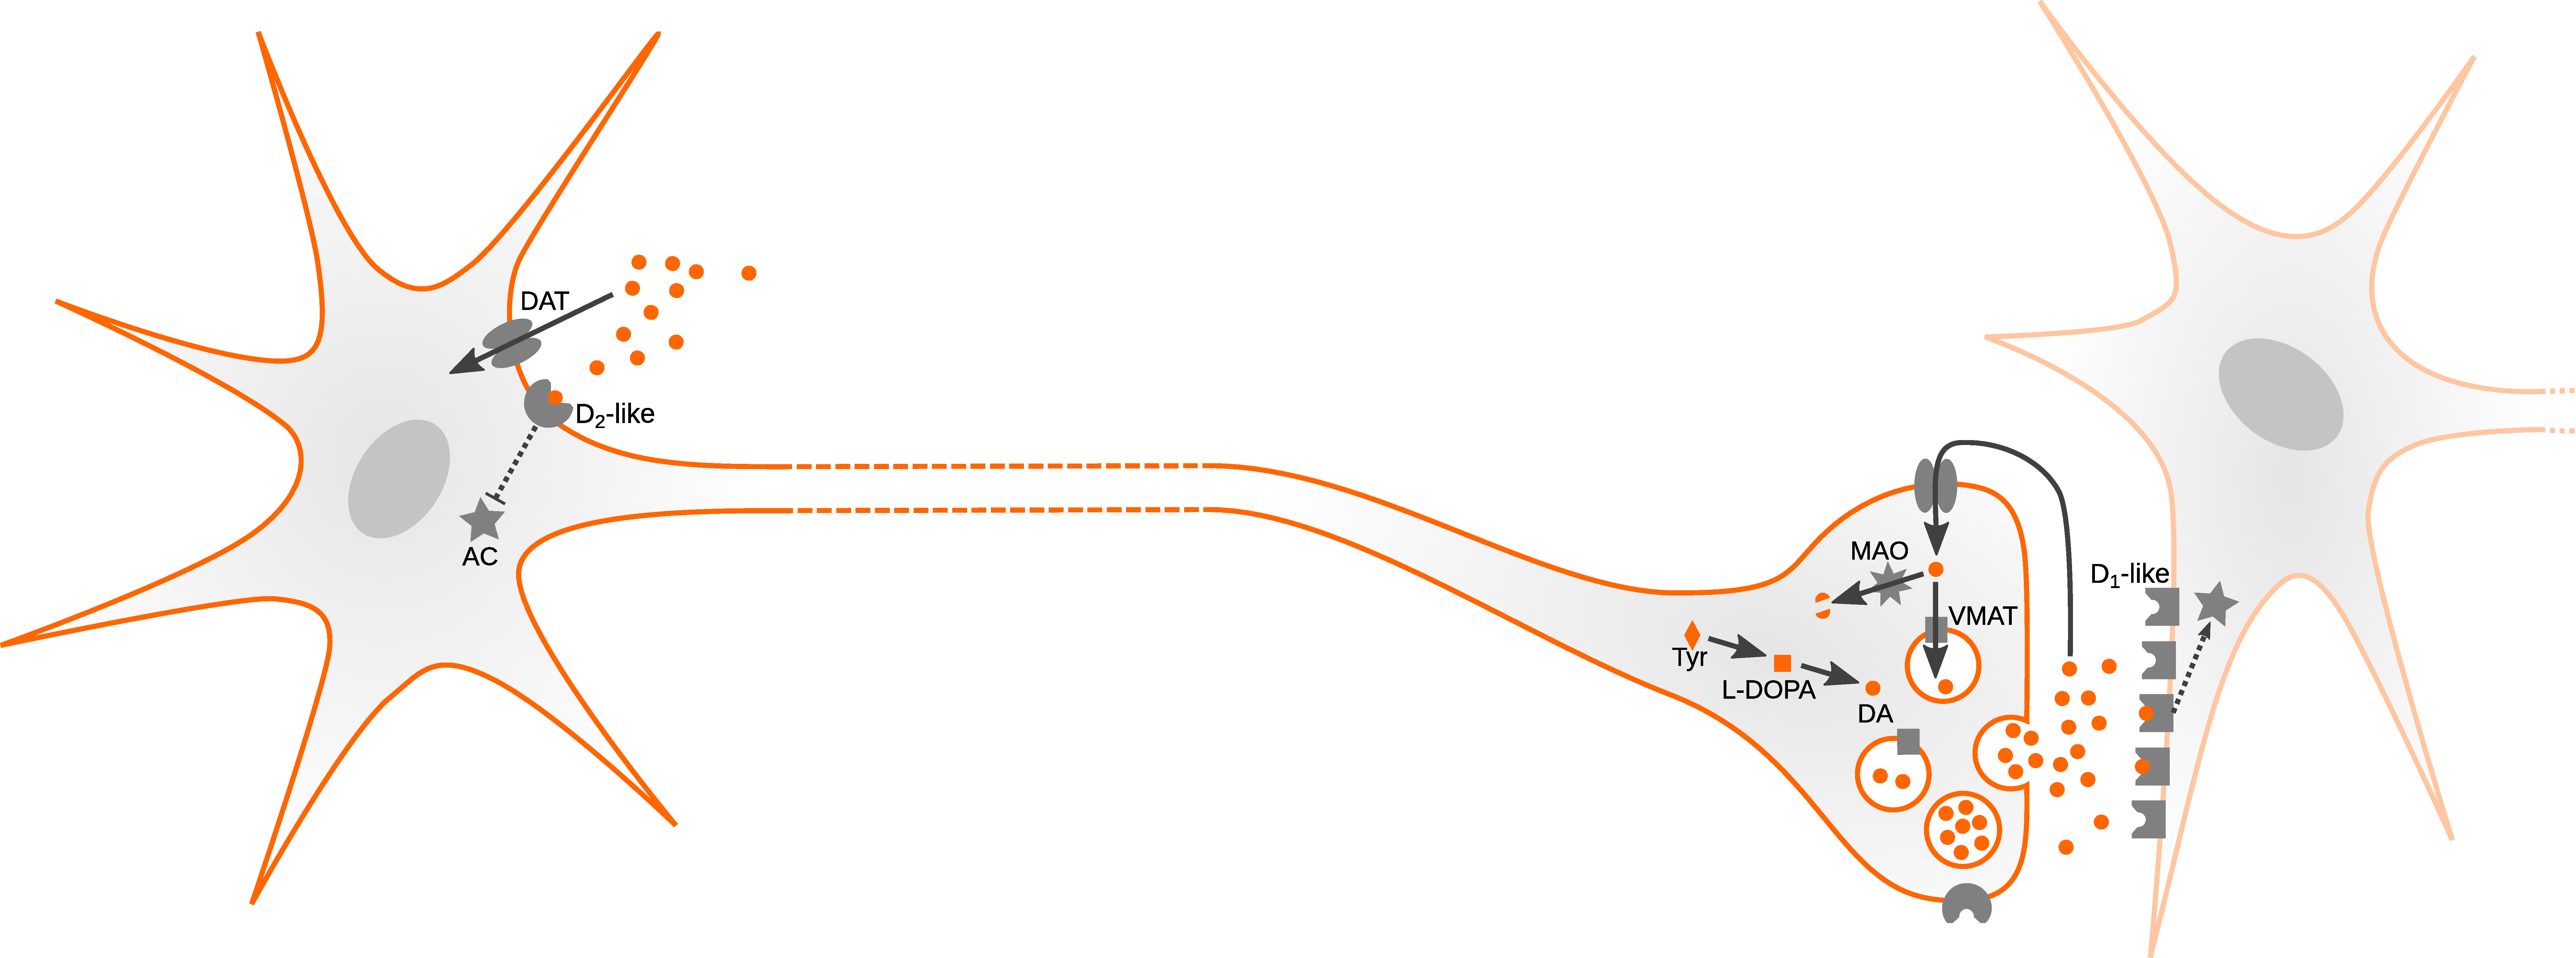
\includegraphics[width=\textwidth]{img/da}
		\caption{
			Schematic overview of VTA dopaminergic neurons, with the soma located in the VTA and synapses in one or multiple other projection area voxels.
			Excitability at the soma are contingent on $\mathrm{D_2}$ autoinhibition, while transmission at the synapse is contingent on dopamine metabolism, turnover, and postsynaptic $\mathrm{D_1}$ expression.
			Abbreviations: AC (adenylyl cyclase), DA (dopamine), DAT (dopamine transporter), MAO (monoamine oxydase), VMAT (vesicular monoamine transporter), Tyr (tyrosine) \cite{Torres2003}.
			}
		\label{fig:cm}
	\end{subfigure}
	\begin{subfigure}{.985\textwidth}
		\centering
		\vspace{.5em}
		\includegraphics[width=0.95\textwidth]{img/optogenetics}
		\caption{
			Schematic of optogenetic cell selection and activation.
			Orange denotes dopaminergic cells, gray enlarged elements on the cell periphery indicate channelrhodopsin expression, and cyan segments on the cell periphery denote depolarization events.
			}
		\label{fig:og}
	\end{subfigure}
	\caption{
		\textbf{The cell biological compartmentalization of dopaminergic neurotransmission (and susceptibility to psychopharmacology) can partly be mapped onto neuroanatomical features by a simple network model, using optogenetics.}
		Depicted are schematic overviews of the VTA dopaminergic system at various spatial resolutions.
		}
	\label{fig:m}
\end{figure*}
\end{sansmath}

\begin{sansmath}
\sessionpy{pytex_subfigs(
        [
                {'script':'scripts/taskgroup.py', 'conf':'article/2x1.conf', 'options_pre':'{.48\\textwidth}',
                        'caption':'Task group comparison for animals targeted at all explored combinations of implant coordinates.',
                        'label':'mvt',
                        },
                {'script':'scripts/implant_coordinates_block.py', 'conf':'article/2x1_coordinates.conf', 'options_pre':'{.48\\textwidth}',
                        'caption':'Implant coordinate comparison for block stimulation trials (inner dots indicate best category group).',
                        'label':'mvib',
                        },
                ],
        caption='
                \\textbf{VTA activation is sensitive to the stimulation protocol category and the implant coordinates, with different trends in block and phasic stimulation trials.}
                Depicted are multifactorial (protocol and implant coordinates) comparisons of signal intensity in the VTA region of interest.
                Abbreviations:
                n (sample size),
                PA (posteroanterior),
                rel. (relative to).
                ',
        label='fig:mv',
        )}
\end{sansmath}

\begin{sansmath}
\sessionpy{pytex_subfigs(
        [
                {'script':'scripts/map_block_filtered_controlled.py', 'conf':'article/2asymetric_map.conf',
                        'options_pre':'{.39\\textwidth}',
                        'options_pre_caption':'\\vspace{-.5em}',
                        'caption':'Second-level t-statistic map for block-stimulus-evoked activity in best implant group animals (corrected for the wild type control response).\\vspace{.5em}',
                        'label':'mbfc',
                        },
                {'script':'scripts/distributions_block_filtered_controlled.py', 'conf':'article/2asymetric_distributions.conf',
                        'options_pre':'{.595\\textwidth}\\vspace{-.4em}',
                        'options_pre_caption':'\\vspace{-2em}',
                        'caption':'Distribution densities of statistic values from block-stimulus-evoked activity analysis in best implant group animals (corrected for the wildtype control response). Depicted are the 10 most strongly activated areas.',
                        'label':'dbfc',
                        },
                {'script':'scripts/map_block_other_controlled.py', 'conf':'article/2asymetric_map.conf',
                        'options_pre':'{.39\\textwidth}',
                        'options_pre_caption':'\\vspace{-.5em}',
                        'caption':'Second-level t-statistic map for block-stimulus-evoked activity in rejected implant group animals (corrected for the wild type control response).\\vspace{.5em}',
                        'label':'mboc',
                        },
                {'script':'scripts/distributions_block_other_controlled.py', 'conf':'article/2asymetric_distributions.conf',
                        'options_pre':'{.595\\textwidth}\\vspace{-.4em}',
                        'options_pre_caption':'\\vspace{-2em}',
                        'caption':'Distribution densities of statistic values from block-stimulus-evoked activity analysis in rejected implant group animals (corrected for the wild type control response). Depicted are the 10 most strongly activated areas.',
                        'label':'dboc',
                        },
                {'script':'scripts/map_block_filtered_seed.py', 'conf':'article/2asymetric_map.conf',
                        'options_pre':'{.39\\textwidth}',
                        'options_pre_caption':'\\vspace{-.5em}',
                        'caption':'Second-level t-statistic map for VTA seed-based functional connectivity during block stimulation in best implant group animals (VTA region in green).\\vspace{.5em}',
                        'label':'mbfs',
                        },
                {'script':'scripts/distributions_block_filtered_seed.py', 'conf':'article/2asymetric_distributions.conf',
                        'options_pre':'{.595\\textwidth}\\vspace{-.4em}',
                        'options_pre_caption':'\\vspace{-2em}',
                        'caption':'Distribution densities of statistic values from seed-based functional connectivity analysis of best implant group animal block stimulation scans. Depicted are the 10 most strongly activated areas.',
                        'label':'dbfs',
                        },
                ],
        caption='
                \\textbf{Block stimulation elicits strong ventral striatal activity in the best implant group, more rostrally weighted activity in the rejected implant group, and generates similar but weaker contrasts for VTA seed-based analysis.}
                The figures show volumetric population t-statistic maps \\textbf{(\subref{fig:mbfc}, \subref{fig:mbfs}, \subref{fig:mboc})} thresholded at $\mathrm{t \geq 3}$ and centered on the VTA target, as well as a break-down of activation along atlas parcellation regions \\textbf{(\subref{fig:dbfc}, \subref{fig:dboc}, \subref{fig:dbfs})}.
                ',
        label='fig:m',
        options_pre='\\centering',
        )}
\end{sansmath}

\begin{sansmath}
\vspace{-.5em}
\sessionpy{pytex_subfigs(
        [
                {'script':'scripts/features_correlation_rois.py', 'conf':'article/1col.conf', 'options_pre':'{.49\\textwidth}\\vspace{-1.5em}',
                        'caption':'
                                Region-wise regression plot between functional and structural projection maps.
                                Tinted area indicates the \\SI{99}{\percent} confidence interval of the regression estimate.
                                ',
                        'label':'fcr',
                        'figure_format':'pdf',
                        },
                {'script':'scripts/features_correlation_voxels.py', 'conf':'article/1col_with_margins.conf', 'options_pre':'{.49\\textwidth}\\vspace{-1.5em}',
                        'caption':'
                                Voxel-wise regression plot between functional and structural projection maps.
                                Tinted area indicates the \\SI{99}{\percent} confidence interval of the regression estimate.
                                ',
                        'label':'fcv',
                        'figure_format':'pdf',
                        },
                {'script':'scripts/features_filtered_coronal.py', 'conf':'article/coronal.conf', 'options_pre':'{\\textwidth}',
                        'caption':'
                                Coronal slices, showing the population-level contrast t-statistic between VTA functional activation and VTA structural projections.
                                ',
                        'options_post':'\\vspace{1.8em}',
                        'label':'ffc',
                        },
                {'script':'scripts/distributions_features_filtered_neg.py', 'conf':'article/2x1_distributions.conf',
                        'options_pre':'{.49\\textwidth}\\vspace{-1.6em}',
                        'options_pre_caption':'\\vspace{-.8em}',
                        'caption':'
                                Distribution densities of t-statistics, showing the regions where VTA structural projection exceeds functional activation most strongly.
                                ',
                        'label':'dffn',
                        },
                {'script':'scripts/distributions_features_filtered_pos.py', 'conf':'article/2x1_distributions.conf',
                        'options_pre':'{.49\\textwidth}\\vspace{-1.6em}',
                        'options_pre_caption':'\\vspace{-.8em}',
                        'caption':'
                                Distribution densities of t-statistics, showing the regions where VTA functional activation exceeds structural projection most strongly.
                                ',
                        'label':'dffp',
                        },
                ],
        caption='
                \\textbf{Comparing VTA functional activation to structural projection data reveals good correspondence, with deviations involving the dorsomedial striatum and the contralateral ventral striatum.}
                Depicted are correlation analyses \\textbf{(\subref{fig:fcr}, \subref{fig:fcv})} of the population-level functional and structural statistic scores, alongside statistic distributions \\textbf{(\subref{fig:ffc}, \subref{fig:dffn}, \subref{fig:dffp})} for the contrast, taking into account variability across subjects.
                Abbreviations:
                Ant. (Anterior),
                EC (Endopiriform Claustrum),
                Int. (Intermediate),
                Med. (Medial),
                Nc. (Nucleus),
                p. (Pars),
                Post. (Posterior),
                WM (White Matter),
                ',
        label='fig:f',
        options_pre='\\centering\n\\vspace{-2em}',
        )}
\end{sansmath}

\begin{figure*}[h!]
	\begin{subfigure}{.269\textwidth}
		\centering
		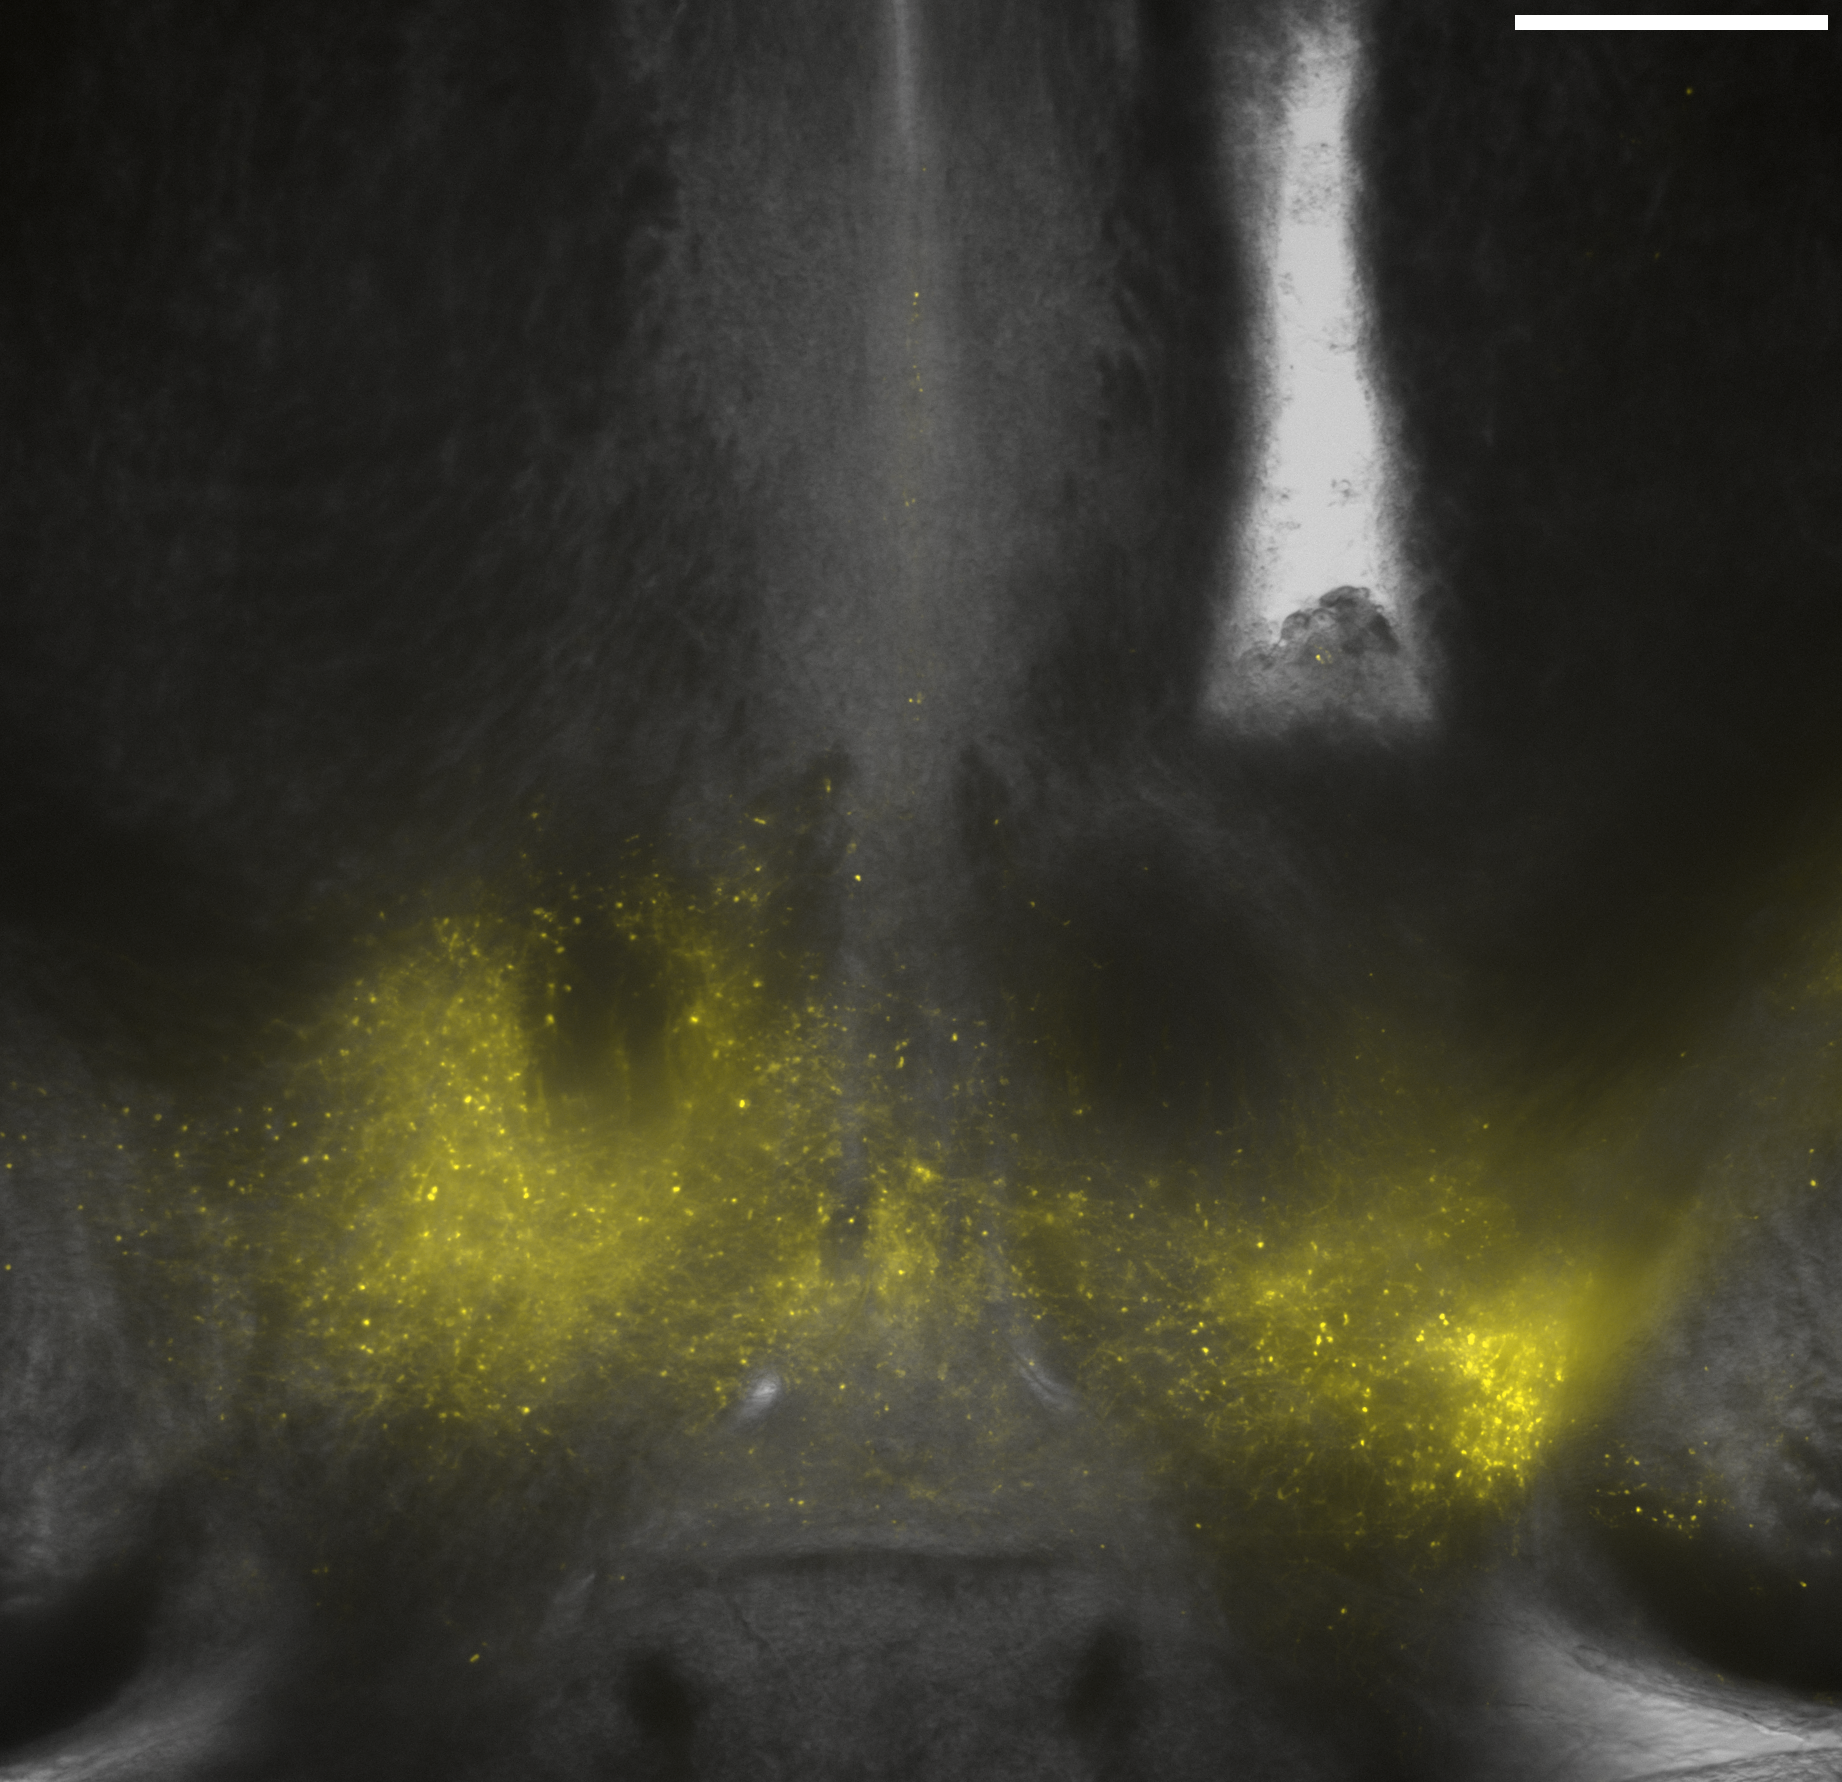
\includegraphics[width=\textwidth]{img/sub-6591_slice-b1_zoom-5_scene-3_transmission-yfp-comb_straight.png}
                \caption{\SI{3.05}{\milli\meter} caudal of Bregma.}
                \label{fig:h6591}
	\end{subfigure}
	\begin{subfigure}{.43\textwidth}
		\centering
		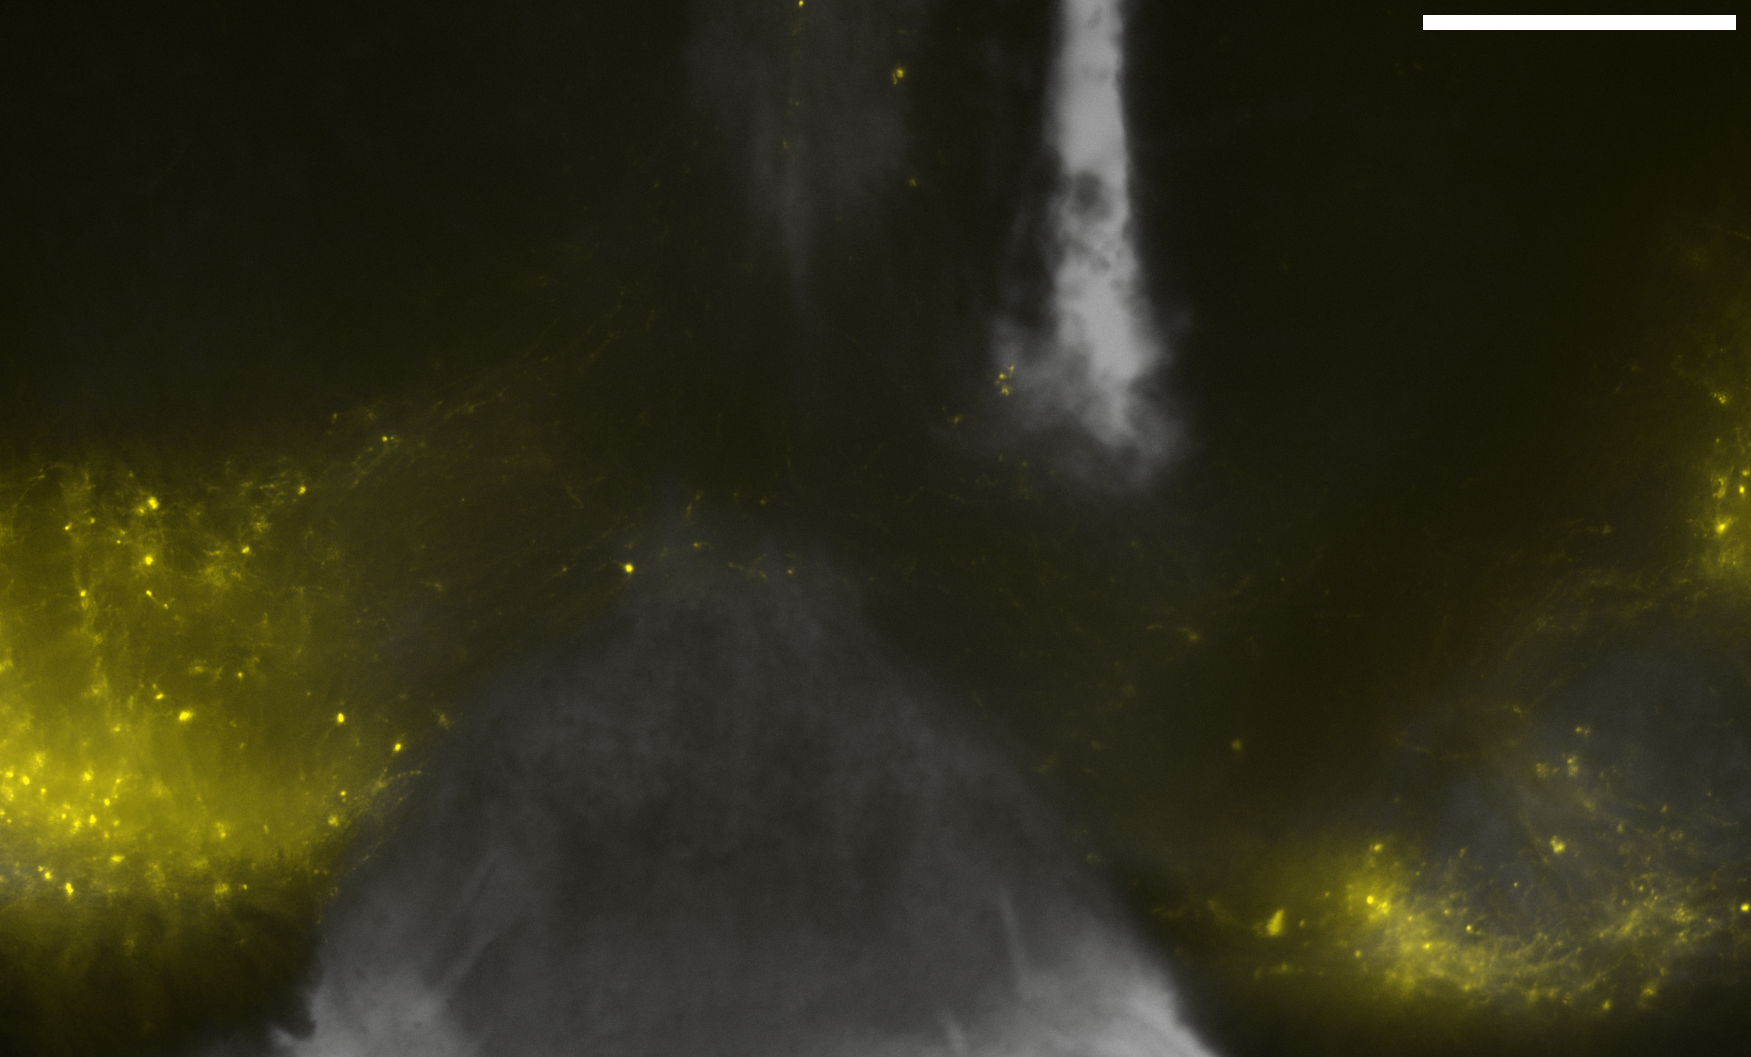
\includegraphics[width=\textwidth]{img/sub-6589_slice-a4_zoom-5_scene-2_transmission-yfp-comb_straight.png}
                \caption{\SI{3.5}{\milli\meter} caudal of Bregma.}
		\label{fig:h6589}
	\end{subfigure}
	\begin{subfigure}{.2728\textwidth}
		\centering
		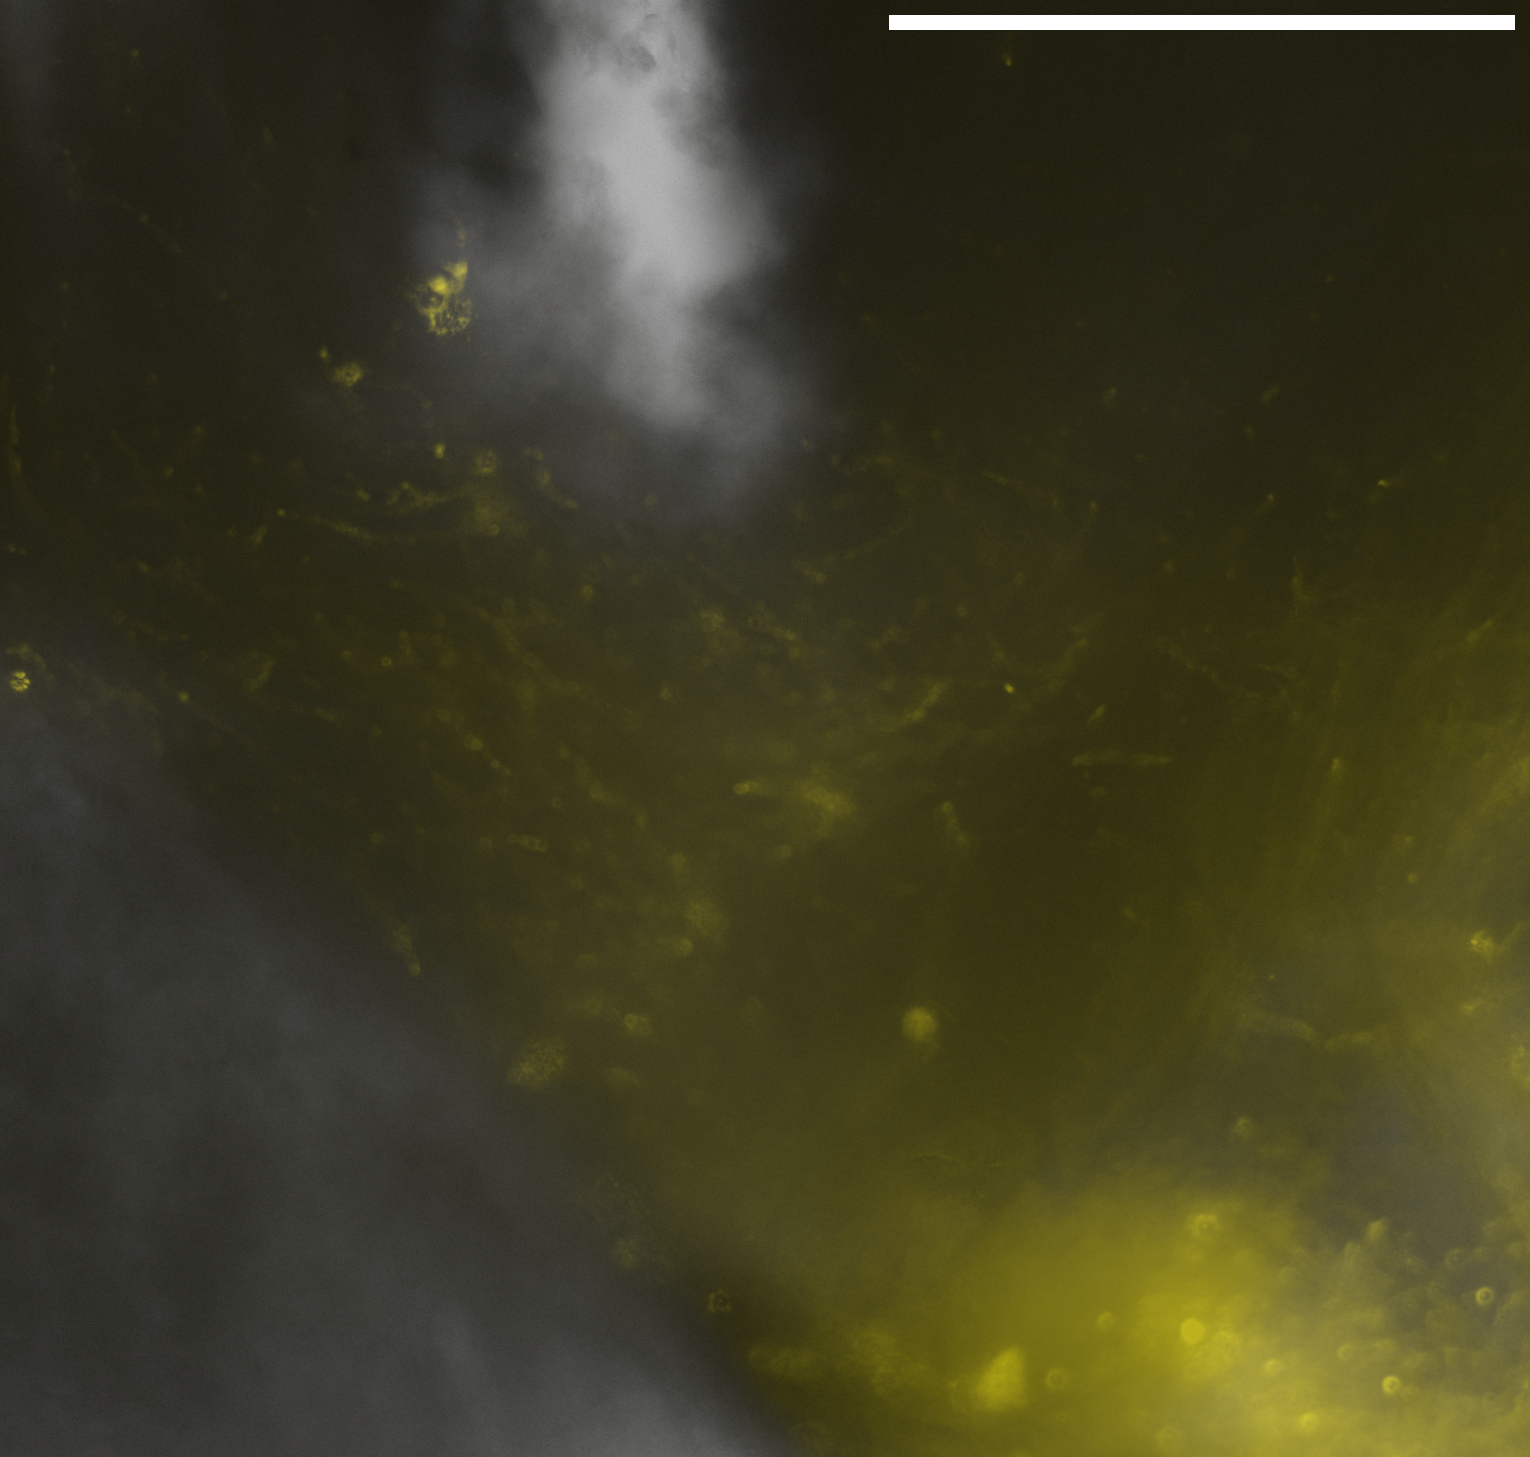
\includegraphics[width=\textwidth]{img/sub-6589_slice-a4_zoom-10_scene-2_transmission-yfp-comb_straight.png}
                \caption{\SI{3.5}{\milli\meter} caudal of Bregma.}
		\label{fig:h6589z}
	\end{subfigure}
        \vspace{-.5em}
	\caption{
		\textbf{Fiber implantation causes strong local cell displacement in the VTA.}
                Depicted are YFP (coexpressed with Channelrhodopsin) fluorescent microscopy images of the VTA, overlaid on corresponding transmission microscopy images of the same focal plane.
                All slices are seen in neurological orientation (the right of the image corresponds to the right of the animal).
                A higher magnification of \textbf{(\subref{fig:h6589})} is depicted in \textbf{(\subref{fig:h6589z})}.
                White bars indicate a scale of \SI{500}{\micro\meter}, and slices are shown in neurological orientation.
                }
	\label{fig:h}
\end{figure*}
